\documentclass{report}
\usepackage{filecontents}

\usepackage[utf8]{inputenc}
\usepackage[T1]{fontenc}
\usepackage[francais]{babel}
\usepackage{listings}
\usepackage[a4paper]{geometry}
\usepackage{graphicx}
\usepackage[export]{adjustbox}
\usepackage{titlesec}
\usepackage{color}
\usepackage[toc, page]{appendix}
\usepackage{url}

\definecolor{xcodekw}{rgb}{0.75, 0.22, 0.60}
\definecolor{xcodestr}{rgb}{0.89, 0.27, 0.30}
\definecolor{xcodecmt}{rgb}{0.31, 0.73, 0.35}

\titleformat{\chapter}[display]
  {\centering\normalfont\huge\bfseries}
  {\chaptertitlename\ \thechapter}
  {20pt}
  {\Huge}

\geometry{hscale=0.75,vscale=0.85,centering}

\renewcommand{\thesection}{\arabic{section}}
\renewcommand\appendixtocname{Annexes}
\renewcommand\appendixname{Annexes}
\renewcommand\appendixpagename{Annexes}

\title{Sécurité des Réseaux Informatiques\\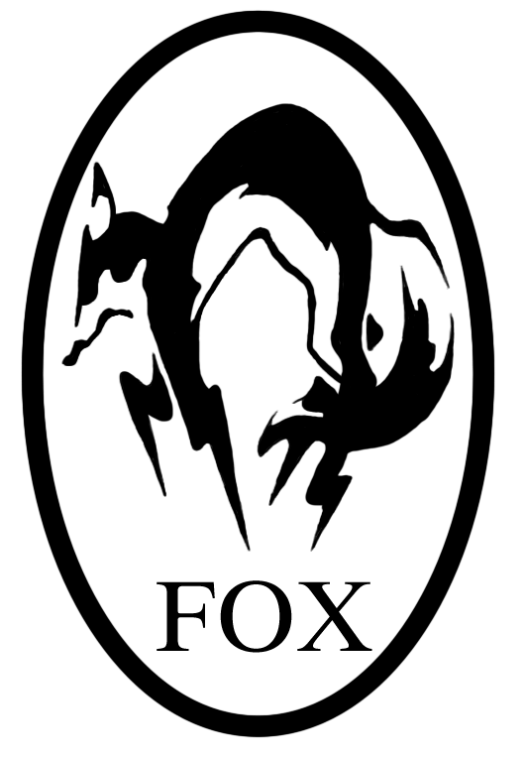
\includegraphics[scale=0.3]{foxhound.png}}
\author{Samuel "Big Boss" \bsc{Monroe}}

\date{30 Mai 2015}

\begin{document}

\maketitle

\newpage
\thispagestyle{empty}
\mbox{}

\tableofcontents

%% \textbf{}

\chapter{Avant-propos}

	Ceci ne consitue pas une synthèse, mais plutôt une oeuvre composée de mes notes prises en cours, et de la réunion du syllabus de V.Van den Schrieck ainsi que du livre Computer Security de Stallings.\\

	Le but est d'obtenir une compréhension totale du cours à la première lecture et d'offrir aux membres de Fox Hound les compétences qui sont attendues d'eux, afin de pouvoir pérenniser ce groupe et ses objectifs.\\

\chapter{Généralités}

	Identification des différents concepts et principes de la sécurité informatique.\\

	\section{Concepts de sécurité informatique}

		\textbf{Sécurité Informatique} : Protection fournie à un SI automatisé pour atteindre les objectifs de préservation \textbf{CIA} des ressources (matériel, logiciels, données, etc..) du SI.\\

		\textbf{CIA} est un concept clé dans la sécurité : \\

		\begin{itemize}
			\item \textbf{Confidentiality} : Préserve les autorisations et restrictions sur l'accès à l'information ainsi que sur la vie privée.\\
			\item \textbf{Integrity} : Protection contre la modification ou suppression impropre de données, incluant l'assertion de l'authenticité des données.\\
			\item \textbf{Availability} : Assure la disponibilité et accessibilité sûre aux données et services.\\
		\end{itemize}

		Ces trois concepts forment la triade \textbf{CIA}, aussi représentée en triangle, et indique les trois objectifs de préservation des assets (\textbf{data} \& \textbf{services}).\\
		Cette triade peut être additionnée de deux autres concepts : \\

		\begin{itemize}
			\item \textbf{Authenticity} : Propriété d'être authentique, et capable d'être vérifié et digne de confiance.\\
			\item \textbf{Accountability} : Besoin de pouvoir tracer les actions à des fins d'identification.\\
		\end{itemize}

	\section{Terminologie}

		Voyons ici quelques termes reliés à la sécurité qu'il est nécéssaire de maîtriser : \\

		\subsection{Asset}

			Les assets, ressources, sont des éléments que les utilisateurs ou propriétaires souhaitent protéger.\\

			Les assets peuvent être \textbf{hardware}, \textbf{software}, \textbf{données} et \textbf{réseux et moyens de communications}. Des ressources non physiques telles que la \textbf{réputation} doivent également être prises en compte.\\

		\subsection{Security Policy}

			Une \textbf{politique de sécurité} est un ensemble de règles ou pratiques qui spécifient ou régulent la manière dont un système ou organisation fournit des services de sécurité pour protéger les \textbf{assets}.\\

			Composée de \textbf{contre-mesures}, ensemble de \textbf{règles} et de \textbf{procédures}.\\

		\subsection{Vulnerability}

			Faille ou faiblesse dans la conception, implémentation, opération ou gestion d'un système, qui peut être \textbf{exploitée} pour violer la \textbf{security policy}.\\

			Ces vulnérabilités peuvent être la \textbf{corruption système} (I) , des \textbf{fuites} (C) ou des \textbf{indisponibilités} (A).\\

		\subsection{Threats and Attacks}

			Une \textbf{menace} est un danger potentiel de sécurité pour une ressource.\\

			L'\textbf{attaque} est la réalisation de ce danger potentiel.\\
			Elles peuvent êtres \textbf{actives} ou \textbf{passives} selon qu'elles altèrent le système ou non, et \textbf{internes} ou \textbf{externes} selon la position de l'attaquant par rapport à l'entreprise.\\

		\subsection{Countermeasures}

			La \textbf{contremesure} est une action visant à réduire une menace, vulnérability ou attaque via prévention, élimination.\\

		\subsection{Risk}

			Le \textbf{risque} est la prévision d'une perte exprimée par la probabilité qu'une menace particulière exploire une vulnérabilité particulière avec un résultat négatif particulier.\\

			Un risque est \textbf{évalué} par la \textbf{probabilité que l'incident} survienne multiplié par \textbf{l'impact} que cet incident causerait.\\

	\section{Menaces, attaques et actifs}

		\subsection{Divulgation non autorisée - Unauthorised Disclosure}

			Menace sur \textbf{Confidentiality}, attaques liées : \\

			\begin{itemize}
				\item \textbf{Exposition} : Exposition d'informations sensibles
				\item \textbf{Interception} : Interception d'informations dans une communication
				\item \textbf{Inférence} : Accession à des infos sensibles de manière indirecte
				\item \textbf{Intrusion}\\
			\end{itemize}

		\subsection{Tromperie - Deception}

			Transmission de fausses infos à une entité en faisant croire que les infos sont conformes. \\

			\begin{itemize}
				\item \textbf{Masquerade} : Accès au système et agissement malicieux sous couvert d'une entité autorisée
				\item \textbf{Falsification} : Alteration de données valides
				\item \textbf{Répudiation}\\
			\end{itemize}

		\subsection{Perturbations - Disruptions}

			Menaces sur \textbf{Availability} et \textbf{Integrity}.\\

			\begin{itemize}
				\item \textbf{Neutralisation} : Destruction physiques ou endommagement du matériel
				\item \textbf{Corruption}
				\item \textbf{Obstruction} : Interruption d'un service, DoS\\
			\end{itemize}

		\subsection{Usurpation}

			Prise de contrôle d'un service ou système par une entité non autorisée.\\

			\begin{itemize}
				\item \textbf{Détournement} : Entité contrôle les ressoruces d'un système
				\item \textbf{Mauvais usage} : Composant système effectue une opération au détriment de la sécurité.\\
			\end{itemize}

	\section{Principes de conception de systèmes sécurisés}

		Pas de techniques pour empêcher totalement des \textbf{failles}, mais des principes existent pour tendre vers un \textbf{système sécurisé} : \\

		\begin{itemize}
		 	\item \textbf{Economy of Mechanisms} : Solutions les moins complexes possibles pour éviter les failles (\textbf{KISS}).\\
		 	\item \textbf{Fail-Safe Default} : Comportement d'exclusion par défault
		 	\item \textbf{Complete Mediation} : Chaque accès système doit être validé, pas de caches
		 	\item \textbf{Open Design} : Elements de conception publiques
		 	\item \textbf{Separation of Privilege}
		 	\item \textbf{Least Privilege} : Droits minimum suffisant pour la tâche
		 	\item \textbf{Least Common Mechanisms} : Il faut minimiser les éléments partagés par les différents programmes ou utilisateurs.
		 	\item \textbf{Psychological Acceptability} : Les mécanismes de sécurité ne doivent pas interférer sans raison avec les tâches des users, qui pourraient les désactiver.
		 	\item \textbf{Isolation} : Systèmes publiques isolés des critques, processus et fichiers utilisateurs isolés de ceux des autres, accès aux mécanismes isolés
		 	\item \textbf{Encapsulation} : Isolation appliquée à l'orienté-objet
		 	\item \textbf{Modularity} : Partage des fonctions et services de sécurité pour une seule implémentation d'un prtocole de sécurité.
		 	\item \textbf{Layering} : Plusieurs couches de protection
		 	\item \textbf{Least Astonishment} : Une GUI doit se comporter comme l'attendrait un utilisateur\\
		 \end{itemize} 

	\section{Stratégies de sécurité informatique}

		Trois étapes pour mettre au point une stratégie : \\

		\begin{enumerate}
			\item \textbf{Définir} la politique de sécurité
			\item \textbf{Implémenter} la politique
			\item \textbf{Valider} la politique\\
		\end{enumerate}

		\subsection{Politiques de sécurité}

			Il faut dans un premier temps définir les \textbf{assets} à protéger et leur \textbf{valeur} qui peut être définie en termes d'objectifs \textbf{CIA}.\\

			Ensuite, il faut identifier les \textbf{vulnérabilités} et \textbf{attaques} potentielles, ainsi que leur \textbf{probabilité} de survenir, et l'\textbf{impact} qu'elles causeraient.\\

			Pour chaque \textbf{vulnérabilité}, on peut mettre en place un série de contre-mesures, dont le choix s'établit sur des compromis tels que la \textbf{facilité d'utilisation et la sécurité}, ainsi que le rapport entre \textbf{coût de la mesure et coût des pertes}.\\

			Les policies sont une décision \textbf{stratégique importante}, chaque choix est un renoncement.\\
			Il faut lister les risques pour lesquels de conte-mesures ne sont pas prises, appelés \textbf{risques résiduels}.\\

		\subsection{Mise en place des contre-mesures}

			Implémentation des mécanismes de sécurité impliques quatre groupes d'actions complémentaires : \\

			\begin{enumerate}
				\item \textbf{Prévention} : Permet de restreindre le nombre d'attaques potentielles
				\item \textbf{Détection} : Pas toujours possible d'éviter une attaque, mais il faut pouvoir la détecter pour prendre action
				\item \textbf{Réaction} : Que faire en cas d'une attaque découverte pour en minimiser les conséquences
				\item \textbf{Récupération} : Comment réagir suite à une perte (backups, etc...)\\
			\end{enumerate}

		\subsection{Validation}

			Le bon fonctionnement du système de sécurité doit être évalué et analysé, il faut donc établir des procédures de validation pour ce faire.\\

	\section{Connaître Son Ennemi}

		Important de connaître l'adversaire pour savoir ce qu'il recherche, ses buts et méthodes et s'en protéger.\\

		\subsection{Types d'attaquants}


			\begin{itemize}
				\item \textbf{Attaques Automatisées} : Virus et vers conçus pour se propager automatiquement sur internet.

				\item \textbf{Scripts Kiddies} : Amateurs utilisants des scripts afin d'expérimenter.

				\item \textbf{Vandale} : Attaquant souhaitant montrer ce dont il est capable pour sa réputation.

				\item \textbf{Activiste} : Attaquant expérimenté ciblant des entités pour raisons politiques.

				\item \textbf{Expert} : Tente de mettre en évidence des failles en réalisant les intrusions, pas de but de destruction.

				\item \textbf{Espion} : Professionel disposant d'outils et méthodes sophistiqués, attaques sur de longues périodes.

				\item \textbf{Cybercrime Organisé} : Organisations à buts financiers, volent par exemple les numéros de cartes de crédit.

				\item \textbf{Cyberterrorisme} : Groupes d'experts bien organisés, buts terroristes et de destruction.\\
			\end{itemize}

		\subsection{Methodes d'attaques}

			Attaquent des cibles \textbf{aléatoires} ou \textbf{spécifiques}.\\

			Les cibles \textbf{spécifiques} nécéssitent une préparation minutieuse, celles \textbf{aléatoires} sont parfois utilisées comme point d'attaques par rebond.\\

		\subsection{Outils privilégiés}

			Les outils utilisés servent principalement à la collecte d'information.\\

			\begin{itemize}
				\item \textbf{WHOIS} : Infos sur Ip, Domain Name
				\item \textbf{Mailing Lists} : Consultation d'archives avec descriptifs de certains problème et infos techniques précises
				\item \textbf{Social Engineering} : Ingénierie Sociale, le but est d'exploiter les failles humaines afin d'en retirer des informations
				\item \textbf{Port Scan} : Montre les services ouverts
				\item \textbf{OS Fingerprinting} : Permettent d'identifier le type d'OS sur base de réponses, ainsi que versions des services etc, utile pour trouver une cible appropriée pour une faille sur une certaine version d'un logiciel.\\
			\end{itemize}

	\section{Exercices}

		\subsection{Questions de révision}

			\begin{itemize}

				\item \textbf{Définition de la sécurité informatique : } \\

				Protection fournie à un système d'information automatisé pour atteindre les objectifs de préservation de CIA (Confidentiality, Integrity, Availability) des ressources du système d'information (matériels, logiciels, firmwares, données, télécommunications).\\

				\item \textbf{Différence entre attaques passives et actives : }\\

				\textbf{Active : } L'attaque essaie d'altérer le système et ses opérations.\\
				\textbf{Passive :} L'attaquant essaie d'obtenir ou d'utiliser les informations du système sans affecter les ressources.\\

				\item \textbf{Listez et définissez brièvement des attaques actives et passives :}\\

					\begin{itemize}

						\item \textbf{Man in the Middle - Passive} : Attaque ayant pour but d'intercepter les communications entre deux parties sans que ni l'un ni l'autre ne puissent se douter que le canal de communication est compromis.\\

						\item \textbf{Keylogger - Passive} : Type de spyware spécialisé pour espionner les frappes clavier sur l'ordinateur hôte, et pour les transmettre via internet à un pirate pour qu'il les exploite.\\

						\item \tetxbf{Injections SQL - Actif(Passif)} : Type d'exploitation d'une faille de sécurité d'une application interagissant avec une base de données, en injectant une requête SQL non prévue par le système et pouvant compromettre sa sécurité.\\

						\item \textbf{Phishing - Passive} : Technique utilisée par des fraudeurs pour obtenir des renseignements personnels dans le but de perpétrer une usurpation d'identité, ou d'utiliser malicieusement ces informations personnelles (vols d'informations bancaires).\\

						\item \textbf{Denial Of Service - Actif} : Attaque informatique ayant pour but d'empêcher les utilisateurs légitimes d'un service de l'utiliser : Innondation d'un réseau, obstruction d'accès à un service à une personne donnée, envoi de milliards d'octets vers une cible.\\

					\end{itemize}

				\item \textbf{Etapes de mise en place d'une stratégie de sécurité informatique :}\\

					\begin{enumerate}

						\item \textbf{Définir} la politique de sécurité, définir ce que le mécanisme doit faire.\\
						\item \textbf{Implémenter} cette politique, quels mécanismes mettre en place.\\
						Analyser le \textbf{Trade-off} (Coût/Bénéfice), prévention, détection, réaction et récupération, documenter les risques résiduels et assurer la maintenance.\\
						\item \textbf{Valider} cette politique, s'assurer que le mécanisme fonctionne.\\

					\end{enumerate}

				\item \textbf{Selon quels critères va-t-on sélectionner les contre-mesures à appliquer dans le cadre d'une politique de sécurité informatique?}\\

					\begin{itemize}
						\item Le premier choix à faire est un compromis entre la facilité d'utilisation et la sécurité.\\
						\item Deuxièment, il faut évaluer le coût que représenteraient une contre-mesure par rapport aux coût des pertes éventuelles et de la procédure de récupération.\\
					\end{itemize}

			\end{itemize}

	\section{Questions de réflexion}

		\subsection{Exigences d'un distributeur de billets en termes CIA}

			\begin{enumerate}
				\item \textbf{Availability : } Exigence basse, l'indisponibilité du service représenterait au pire un dérangement minimal pour l'utilisateur, car il peut toujours payer ses achats avec sa carte en magasin, manipuler son compte via e-banking, ou éventuellement aller retirer son argent dans un autre ATM d'une autre banque.\\
				\item \textbf{Integrity : } Exigence haute, car une erreur de données au niveau du retrait ou du dépôt de billets pourrait être catastrophique pour l'utilisateur, par exemple si son compte était débité de 500 euros pour un retrait de 50.\\
				L'inverse est valable pour la banque elle-même, dans un cas où les utilisateurs recevraient beaucoup plus que le montant demandé.\\
				\item \textbf{Confidentiality : } Exigence haute, une faille dans la confidentialité serait catastrophique si quelqu'un de mal intentionné pouvait avoir accès au compte de l'utilisateur.\\
				Cette faille aurait aussi un impact considérable sur la réputation de la banque.\\
			\end{enumerate}

		\subsection{Impact d'attaques en termes de CIA sur : }

			\begin{itemize}
				\item \textbf{Organisation avec mise à disposition d'info publiques sur son serveur Web : }\\
					\begin{enumerate}
						\item C : Documents publiques, pas de réel impact puisque disponibles pour tout le monde.
						\item I : Impact faible, les documents étant publiques, un impact sur l'intégrité pourrait gêner les utilisateurs et les possesseurs.\\
						\item A : Impact faible à modéré, tout dépend de l'utilité de ces documents au public, mais si ces données sont publiques c'est qu'elles sont probablement de moindre importance et leur indisponibilité serait au pire gênante pour l'utilisateur.\\
					\end{enumerate}
				\item \textbf{Organisation policière, données exrêmement sensibles pour investigations : }\\
					\begin{enumerate}
						\item C : Les documents étant extrêmement sensibles, l'impact est élevé, toute divulgation pourrait nuire grandement au bon déroulement des enquêtes avec toutes les conséquences que cela entraînerait.\\
						\item I : Leur intégrité est primordiale, pour les mêmes raisons que sus-mentionnées.\\
						\item A : Leur indisponibilité pourrait avoir au pire un impact modéré, tout dépend des échéances de l'enquête.\\
					\end{enumerate}
				\item \textbf{Organisation financière, information administrative de routine : }\\
					\begin{enumerate}
						\item C : Impact modéré, ces informations étant de routines, on peut envisager que leur divulgation serait au pire assez gênante pour l'organisation, mais pas au point de pouvoir mettre en péril ses activités.\\
						\item I : Impact élevé, même si ces informations sont de routines, des erreurs dans ces informations pourraient mener à des chiffres non justes dans les calculs finaux de l'organisation, l'intégrité doit être assurée absolument.\\
						\item A : Impact modéré-élevé : Si ces informations sont dites "de routine", on peut estimer que leur indisponibilité empêcherait le fonctionnement en temps réel de l'organisation sur certains secteurs, situation qui pourrait être dommageable pour celle-ci.\\
					\end{enumerate}
				\item \textbf{Système SCADA - Organisation militaire}
					\begin{enumerate}
						\item C : Impact faible pour les informations de routine, tandis qu'une faille dans la confidentialité des informations de senseurs pourraient avoir un impact élevé si exploités par une nation ennemie ou un groupe terroriste.\\
						\item I : Impact faible pour les informations de routine, probablement élevés pour celles de senseurs.\\
						\item A : Impact faible pour informations de routine, élevés pour celles de senseurs.\\
					\end{enumerate}
			\end{itemize}

		\subsection{Activités considérées comme menace potentielle pour le réseau d'une entreprise, et pourquoi? : }\\
			\begin{itemize}
				\item \textbf{Employé responsable de la distribution interne du courrier : } Menace potentielle, cet employé pourrait par exemple détourner le courrier à destination des supérieurs, ou à destination de certains secteurs sensibles de l'entreprise.\\
				\item \textbf{Anciens employés licenciés pour cause de restructuration : } Certains pouvant sans doutes êtres rancuniers vis-à-vis de la situation vécue, ils pourraient éventuellement essayer de se servir de leurs anciens logins pour causer du tort à l'entreprise, récupèrer des documents sensibles, etc...
				\item \textbf{Employé en voyage d'affaire : } Divulgation d'informations sensibles au cours d'une soirée arrosée.\\
				\item \textbf{Compagnie de gestion des bâtiments : } Les système d'extinction automatiques étant contrôlés par cette compagnie, et pas par l'entreprise, on ne connaît pas le niveau de sécurité de leur système informatique et de leur système de contrôle à distance, quelqu'un ayant accès à cette compagnie pourrait activer ces extincteurs, voir les désactiver.\\
			\end{itemize}

			%%%%%%%%%%%%
			%%% TODO %%%
			%%%%%%%%%%%%

\chapter{Bases de Cryptographie}

	\section{Chiffrement Symétrique}

	\section{Hashage et authenticatio des messages}

	\section{Chiffrement Clé Publique}

	\section{Signatures Digitales}

	\section{Gestion des clés}
	
	\section{Exercices}

		\subsection{Questions de révision}

			\begin{itemize}
				\item \textbf{Quels sont les éléments intervenants dans un chiffrement symétrique ?} \\

					\begin{enumerate}
						\item Le message en clair
						\item L'algorithme de chiffrement
						\item Une clé secrète appliquée à l'algorithme
						\item Le message chiffré
						\item L'algorithme de déchiffrement
					\end{enumerate}

				\item \textbf{Combien de clés faut-il pour que deux personnes puissent communiquer par chiffrement symétrique ?}\\

					Il suffit d'une clé, qui est partagée entre les deux entités communiquantes.\\

				\item \textbf{Quelles sont les deux contraintes principales pour garantir la sécurité du chiffrement symétrique ?}\\

					\begin{enumerate}
						\item Un algorithme de chiffrement fort
						\item L'émetteur et le reçeveur doivent avoir obtenu leur copie de clé de manière sécurisée\\
					\end{enumerate}

				\item \textbf{Listez les trois approches permettant de faire de l'authentification de messages :}\\

					\begin{enumerate}
						\item Le chiffrement des messages via le chiffrement symétrique
						\item Ajout d'un tag en fin de message (MAC) calculé via clé symétrique
						\item Ajout d'un tag via hashage unidirectionnel (signature digitale), plus besoin de clés partagées\\
					\end{enumerate}

				\item \textbf{Quels sont les éléments intervenant dans un chiffrement asymétrique ?}\\

					\begin{itemize}
						\item Le message en clair
						\item L'algorithme de chiffrement
						\item Une clé publique et une clé privée, une pour chiffrer et l'autre déchiffrer
						\item Le message chiffré
						\item L'algorithme de déchiffrement\\
					\end{itemize}

				\item \textbf{Listez et expliquez brièvement trois utilisations d'un cryptosystème à clé publique}\\

					\begin{enumerate}
						\item La signature numérique : On génère le tag qui prouve la validité du message et on le chiffre avec la clé secrète, le receveur regénère ce tag avec sa propre fonction et vérifié le tag reçu en le déchiffrant avec la clé publique.
						\item La distribution de clés symétriques : Si deux entités veulent se communiquer une clé secrète, Alice chiffre la clé secrète à partager avec la clé publique de Bob, Bob reçoit cette clé secrète et la déchiffre avec sa clé privée.
						\item Le chiffrement de clé secrète : Afin de ne pas avoir sa clé secète en clair dans ses fichiers, Bob peut la chiffrer avec une autre clé publique.\\
					\end{enumerate}

				\item \textbf{Quelle est la différence entre une clé privée et une clé secrète ?}\\

					La clé privée fait partie du système de chiffrement asymétrique, elle est utilisable pour déchiffrer des messages chiffrés avec la clé publique qui lui est paire, tandis que la clé secrète est conçue pour chiffrer \textbf{et} déchiffrer un même message.\\

				\item \textbf{Qu'est-ce qu'une signature numérique ?}\\

					C'est un tag ajouté au message afin de prouvé sa validité, il est généré en calculant une valeur \textbf{hashée} du message, en chiffrant ce hash avec sa clé privée.\\
					Ce hash chiffré accompagnera le message, sera déchiffrable en utilisant la clé publique de l'émetteur.\\
					Le hash déchiffré sera comparé à un hash généré côté émetteur, leur correspondance prouvera que le message n'a pas été altéré.\\

				\item \textbf{Qu'est-ce qu'un certificat de clé publique ?}\\

					C'est un certificat géré par une Autorité Certificative qui est composé de l'identifiant d'un tiers et de sa clé publique, et prouve son identité. Cela évite l'utilisation par masquarade d'une clé publique de quelqu'un d'autre.\\

				\item \textbf{Comment le chiffrement à clé publique peut-il être utilisé pour distribuer une clé secrète?}\\

					Alice chiffre la clé secrète avec la clé publique de Bob, Bob reçoit le message chiffré, lui seul peut le déchiffrer avec sa clé privée.\\
					Bob et Alice possèdent maintenant tous deux la clé privée.\\

				\item \textbf{Faites un schéma expliquant le mécanisme d'enveloppe numérique}\\

					\textbf{TODO}

			\end{itemize}

		\subsection{Questions de réflexion}

			\begin{enumerate}
				\item \textbf{On cherche un moyen de s’assurer que vous et une autre personne êtes en possession de la même clé secrète, sans transmettre cette clé. On vous propose de créer une chaîne de bits aléatoire ayant la longueur de la clé, d’effectuer un XOR entre cette chaîne et la clé secrète, puis d’envoyer le résultat à l’autre personne. Cette dernière effectue un XOR entre ce qu’il a reçu et sa clé secrète et renvoie le résultat. Vous pouvez alors vérifier que la chaine renvoyée correspond bien à la chaîne aléatoire que vous avez générée pour vous assurer que votre correspondant possède bien la même clé que vous. Que pensez-vous de la sécurité de ce mécanisme ?}\\

					Ce n'est pas sécurisé, en faisant un XOR des deux messages qui transitent entre les deux entités, on retrouve la clé secrète.\\

				\item \textbf{Comment pourrait-on ajouter un mécanisme d’authentification au système d’enveloppe numérique ? Faites un schéma.}\\

					Génération de deux signatures digitales. \textbf{TODO}

					Génération d'une signature digitale sur l'enveloppe elle-même.


			\end{enumerate}

\chapter{Authentification de l'utilisateur}
	
	\section{Exercices}

		\subsection{Questions de révision}

			\begin{itemize}
				\item \textbf{Décrivez en termes généraux quatres moyens pour authentifier l'identité d'un utilisateur}\\

					\begin{enumerate}
						\item L'identification par mots de passes
						\item Token
						\item Biométrique
						\item A distance\\
					\end{enumerate}

				\item \textbf{Listez et décrivez brièvement les menaces principales au secret des mots de passe}\\

					\begin{itemize}
						\item Attaque par dictionnaire hors-ligne : Accès au fichier mot de passe, craquage brute-force sur ce fichier (John The Ripper).
						\item Attaque sur un compte spécifique : Essais de combinaisons de logins/mot de passe.
						\item Attaque par mot de passe populaire : Essai de logins avec les mots de passes fréquemments utilisés.
						\item Piratage du poste de travail
						\item Social Engeneering
						\item Exploitation de l'usage multiple d'un mot de passe
						\item Surveillance électronique\\
					\end{itemize}

				\item \textbf{Comment peut-on protéger un fichier de mot de passe? Pourquoi est-ce important?}\\

					Premièrement via le hashage - salage des mots de passes, et ensuite en les stockant dans un fichier \textbf{shadow} situé dans les fichiers root, qui nécéssitent donc des droits d'administrations pour être accédés.\\
					C'est important car un fichier de mots de passes peut-être utilisé avec un cracker dictionnaire pour en déloger les mots de passes hashés.\\

				\item \textbf{Listez et décrivez brièvement quatre techniques qui permettent de garantir que les mots de passes d'un système sont sécurisés}\\

					\begin{enumerate}
						\item Sensibilisation des utilisateurs
						\item Génération automatiques des mots de passes
						\item Vérification des mots de passes
						\item Vérification proactive des mots de passes\\
					\end{enumerate}

				\item \textbf{Quelle est la différence entre une carte à mémoire et une smart card ?}\\

					Carte-mémoire : 
					\begin{itemize}
						\item Nécéssitent lecteur spécial
						\item Associé à un code
						\item Perte du token signifie risque de sécurité\\
					\end{itemize}

					Smart-Card :
					\begin{itemize}
						\item La plupart du temps générent un identifiant pour accèder au système, le token n'est donc pas l'objet direct d'authentification
						\item La perte de la smart-card n'implique pas de risques de sécurité\\
					\end{itemize}

				\item \textbf{Listez les principales caractéristiques physiques utilisées pour l'authentification biométrique}\\

					\begin{enumerate}
						\item Reconnaissance faciale
						\item Empreintes digitales
						\item Géométrie de la main
						\item Empreinte rétinienne
						\item Iris
						\item Signature manuscrite
						\item La voix\\
					\end{enumerate}

			\end{itemize}
				

		\subsection{Questions de réflexion}

			\begin{enumerate}
				\item \textbf{Discutez de l'adéquation des mots de passes suivants :}\\
					\begin{itemize}
						\item 1-EBL-345 : Chiffres, lettres et caractères spéciaux, bon niveau
						\item mfmitm : Peu et niquement lettres bien que pas dans un dictionnaire, faible niveau
						\item Nathalie1 : Prénom + chiffre, très faible niveau
						\item Whashington : Variation d'un nom connu, faible niveau
						\item Aristotle : Nom connu tel quel, très très faible niveau
						\item tv9stove : Niveau moyen, pas de sens et présence de chiffres
					\end{itemize}
			\end{enumerate}

\chapter{Contrôle d'accès}
	
	\section{Exercices}

		\subsection{Questions de révision}
			\begin{itemize}
				\item \textbf{Expliquez le modèle AAA}\\

					Protocole de contrôle d'accès : \\

					\begin{itemize}
						\item \textbf{Authentication} : Vérification de la validité des éléments prouvant l'identité d'une personne ou d'une entité système.
						\item \textbf{Authorization} : Vérifier si la personne identifiée bénéficie des autorisations requises pour accéder au système.
						\item \textbf{Accounting} : Surveillance des accès aux ressources, logs, ...\\
					\end{itemize}

				\item \textbf{Quelles sont les différences entre le modèle DAC, MAC, et RBAC? Donnez un exemple d'utilisation}\\

					\begin{itemize}
						\item \textbf{Discretionary Access Control} : Contrôle d'accès basé sur des règles fixant quels demandeurs sont ou non autorisés à effectué une action, discretionnaire car une entité peut transmettre ses droits. (SQL)
						\item \textbf{Mandatory Access Control} : Contrôle d'accès basé sur le niveau de confidentialité (documents secrets, top secrets) qui est comparé aux droits d'accès du demandeur d'accès. Mandatoire car ces droits ne sont pas transmissibles.
						\item \textbf{Role Based Access Control} : Droits d'accès définis pour des catégories d'utilisateurs.\\
					\end{itemize}

				\item \textbf{Quelle est la différence entre un sujet et un objet dans le contrôle d'accès?}\\

					\begin{itemize}
						\item \textbf{Sujet : } Entité pouvant accéder à des objets.
						\item \textbf{Objet : } Ressource dont l'accès est contrôlé.
					\end{itemize}

				\item \textbf{Listez quelques droits d'accès possibles}\\

					\begin{itemize}
						\item Lecture
						\item Ecriture
						\item Exécution
						\item Suppression
						\item Création
						\item Recherche
					\end{itemize}

				\item \textbf{Expliquez que sont les bits Sticky, SetUID et SetGID dans le système de contrôle d'accès Unix classique.}\\

					\begin{itemize}
						\item \textbf{Sticky Bit : } Indique que seul le propriétaire d'un fichier du répertoire peut renommer, déplacer ou supprimer ce fichier.
						\item \textbf{SetGID : } Indique que les fichiers nouvellement créés seront associés au GID de ce répertoire.
						\item \textbf{SetUID : } Lorsqu'un utilisateur possédant les droits d'exec sur un fichier l'exécute, on lui attribue temporairement les droits du user créateur du fichier.\\
					\end{itemize}

				\item \textbf{Expliquez les droits d'accès Read, Write et Execute dans le cas d'un répertoire}\\

					\begin{itemize}
						\item \textbf{Read : } Droit de listing
						\item \textbf{Write : } Droit de création, renommage, suppresion de fichiers
						\item \textbf{Execute : } Droits de recherche ou de traverser le dossier
					\end{itemize}

				\item \textbf{En quoi est-ce que le bit SetUID peut éventuellement poser problème?}\\

					Mettre un fichier et surtout un programme en Setuid ou Setgid n'est pas anodin car cela court-circuite le système de protection. Ainsi si vous tapez chmod ug+s /bin/bash vous donnez les droits root à toute personne qui ouvre un terminal ou qui lance l'interpréteur de commande bash. \textit{Wikipédia : Setuid}

				\item \textbf{Expliquez brièvement ce que les Access Lists apportent par rapport au système de contrôle d'accès classique Unix}\\

					Le découpage des droits ne se fait plus sur les groupes mais sur les utilisateurs mêmes, une liste données donne tels drois pour tels fichiers à tels users.\\

				\item \textbf{Donnez et expliquez trois bonnes pratiques dans le cadre du contrôle d'accès}	\\

					\begin{itemize}
						\item Interdire l'accès aux utilisateurs non authentifiés
						\item Désactiver les services inutiles
						\item Retirer immédiatement les comptes des personnes qui quittent la société
						\item Bloquer l'accès si trop d'essais infructueux
					\end{itemize}
			\end{itemize}
				

		\subsection{Questions de réflexion}

			\begin{enumerate}
				\item \textbf{TODO}
			\end{enumerate}

\chapter{Sécurité des DB \& Cloud Computing}
	
	\section{Exercices}

		\subsection{Questions de révision}

			\begin{itemize}
				\item \textbf{Expliquez le concept d'autorisation en cascade}

					Si Alice donne à Bob ses droits, Bob peut également les donner à Charlie, qui peut ensuite en donner à Daryl.\\
					Si maintenant on décide de retirer les droits accordés à Bob par Alice, ce retrait va se faire en cascade et Charlie et Daryl vont perdre les droits qu'Alice avait légués par Bob et que lui-même leur avait légué.\\

				\item \textbf{Expliquez l'injection SQL par tautologie}

					On fait en sorte de modifier la requête pour y injecter une condition toujours vraie pour passer outre la vérification de mots de passe.\\

				\item \textbf{Expliquez la menace d'inférence sur une base de données}

					L'attaquant observe la manière dont le système réagit à l'attaque pour en déduire des informations sur son comportement, en essayant par exemple d'afficher des messages d'erreurs trop descriptifs, ou insérant des requêtes SQL à l'aveugle.\\

				\item \textbf{Quels sont les désavantages du chiffrement d'une base de données?}

					Gestion des clés complexes, complexifie et ralenti le process de la base de données (qu'on veut rapide la plupart du temps).

				\item \textbf{Listez et décrivez brièvement les trois modèles du service Cloud}

					\begin{itemize}
						\item \textbf{Software As A Service : } Application logicielle disponible dans le cloud, telle que le client mail GMail
						\item \textbf{Platform As A Service : } Plateforme sur laquelle une organisation peut développer et faire tourer ses propres applications, telle Google App Engine.
						\item \textbf{Infrastructure As A Service : } La ressource est matérielle (machines + OS) contrôlables via une API, tels Windows Azure, DigitalOcean.\\
					\end{itemize}

				\item \textbf{Décrivez trois menaces de sécurité spécifiques au cloud}

					\begin{itemize}
						\item Abus et usage malicieux du Cloud, création d'un botnet de machines dans le cloud.
						\item Interfaces et API non sécurisées.
						\item Pertes ou fuites des données.\\
					\end{itemize}
			\end{itemize}
			

		\subsection{Questions de réflexion}

			\begin{enumerate}
				\item \textbf{TODO}
			\end{enumerate}

\chapter{Malwares}
	
	\section{Exercices}

		\subsection{Questions de révision}

			\begin{itemize}
				\item \textbf{Quels sont les trois modes de propagation de malware ? : }\\

					\begin{itemize}
						\item Via du contenu infecté (\textbf{virus}).
						\item Via l'exploitation de vulnérabilités (\textbf{vers}).
						\item Via techniques de social engineering (\textbf{spams et trojan}).
					\end{itemize}

				\item \textbf{Catégories d'actions qu'un malware peut effectuer : }

					\begin{enumerate}
						\item Corruption des systèmes
						\item Agents d'attaque
						\item Vol d'information
						\item Furtivité
					\end{enumerate}

				\item \textbf{Quelles sont les phases typiques du cycle de vie d'un virus}

					\begin{enumerate}
						\item Sommeil
						\item Propagation
						\item Déclanchement
						\item Exécution
					\end{enumerate}

				\item \textbf{Quel moyen un ver peut-il utiliser pour accéder à des systèmes distants pour se propager ? :}

					\begin{itemize}
						\item Scan aléatoire
						\item Hit-list
						\item Scan topologique
						\item Réseau local
					\end{itemize}
			\end{itemize}

\chapter{Attaques par Déni de Service}
	
	\section{Exercices}

		\section{Questions de révision}

			\begin{itemize}
				\item \textbf{Quels types de ressources sont visés par les attaques DoS? : }\\

					\begin{itemize}
						\item Bande-passant réseau
						\item Ressources système
						\item Ressources applicatives
					\end{itemize}

				\item \textbf{Quel est le but d'une attaque DoS ? :}\\

					Empêcher ou compliquer l'usage légitime de réseaux, systèmes ou applications en saturant les ressources.\\

				\item \textbf{Quels types de paquets sont utilisés pour les attaques DoS? :}\\

					\begin{itemize}
						\item ICMP
						\item TCP
						\item UDP
						\item HTTP	
					\end{itemize}

				\item \textbf{Pourquoi est-ce que beaucoup d'attaques DoS utilisent le spoofing d'adresses? : }\\

					Pour ne pas que l'on puisse remonter à la source de ces attaques.\\

				\item \textbf{Quelles sont les défenses possibles contre les attaques TCP SYN flooding? : }\\

					Identifier l'attaquant.\\

				\item \textbf{Que faut-il faire lorsqu'une attaque DoS est détectée? : }\\

					Filtrer les paquets concernés, collaborer avec le FAI, traçer la source et l'indentifier.\\

				\item \textbf{Qu'est-ce qu'une attaque par réflexion? Et par amplification? :}\\

					\begin{itemize}
						\item Réflexion : Se base sur des relais intermédiaires pour rediriger un flux vers la cible.
						\item Amplification : Rediriger des paquets amplifiés (réponses DNS) sur une IP spoofée.
					\end{itemize}

			\end{itemize}

\chapter{Détection d'intrusion}

	\section{Exercices}

		\subsection{Questions de révision}

			\begin{enumerate}
				\item \textbf{Listez et définissez quatres types d'intrus : }\\

					\begin{enumerate}
						\item \textbf{Cyber-Criminels : } Objectif financier, via vol d'indentité, accès à des organismes financiers, espionnage, vol de données.\\
						\item \textbf{Activistes : } Causes politiques ou sociales, veulent promouvoir leurs causes via Defaces ou DoS Attacks.\\
						\item \textbf{Organisations sponsorisées par un état : } Advanced Persistant Threats, attaques d'espionnage ou de sabotage.\\
						\item \textbf{Autres : } Hackers classiques motivés par le challenge ou la reconnaissances de leurs pairs.\\
					\end{enumerate}

				\item \textbf{Donnez les principales étapes d'une intrusion avec un exemple d'activité : }\\

					\begin{itemize}
						\item \textbf{Choix de la cible} : Scanning NMAP, WhoIS
						\item \textbf{Accès initial} : Crackage de mot de passe, MalWare, Social Engineering
						\item \textbf{Acquisition de privilèges} : Vulnérabilités logicielles ou sniffer pour obtenir un mot de passe
						\item \textbf{Collecte d'informations ou exploitation du système} : Scan de fichiers, obtention de mots de passes vers d'autres réseaux.
						\item \textbf{Pérénnisation de l'accès} : Installation de Backdoors
						\item \textbf{Dissimulation des traces} : Rootkits, modification des logs
					\end{itemize}

				\item \textbf{Quelle est la différence entre un HIDS et un NIDS? Comment peut-on les combiner? }\\

					Un HIDS surveille un hôte uniquement sur base des events qui se produisent dessus, un NIDS surveille le trafic réseau de certains segments ou appareils spécifiques.\\
					On peut les combiner sur in IDS Hybride qui combine ces différents senseurs.\\

				\item \textbf{Quel sera l'impact d'un faux positif avec un NIDS? Et un faux négatif? : }\\

					Trop de faux positifs amènera l'équipe d'administration à les ignorer, un faux négatif sera plus pernicieux car considéré comme légitime et de base moins surveillé qu'un faux positif.\\

				\item \textbf{Quels types de senseurs peut utiliser un HIDS? Et un NIDS? }\\

					Pour un HIDS : \\
					\begin{itemize}
						\item Traces d'appels systèmes 
						\item Fichiers de logs
						\item Checksums d'intégrité des fichiers
						\item Accès au registre\\
					\end{itemize}

					Pour un NIDS : \\
					\begin{itemize}
						\item Détection d'anomalie
						\item Détection par signature
					\end{itemize}

				\item \textbf{Où placer un NIDS? }\\

					\begin{itemize}
						\item Niveau du firewall externe
						\item Extérieur du réseau
						\item Au niveau du backbone du réseau
						\item Au niveau du LAN et machines spécifiques
					\end{itemize}

				\item \textbf{Qu'est-ce qu'un honeypot? }\\

					Un leurre conçu spécifiquement pour attirer les auteurs d'attaques et les distraire, collecter des infos sur ces attaques et les retenir assez longtemps pour permettre une réaction de l'administrateur.
			\end{enumerate}
\end{document}


